% !TeX spellcheck = en_US
\chapter{State of Science and Technology}%
The following chapter gives an overview of manufacturing technologies, CAM, and various algorithms for optimization problems. Special attention is given to the comparison of optimization problems in manufacturing with redundant degrees of freedom. 


\section{Manufacturing Technologies}
Manufacturing technologies encompass a wide range of processes that are used to transform raw materials into finished products. Two major categories within this field are subtractive and additive manufacturing~\cite{Iqbal.2020}. Subtractive manufacturing involves removing material from a workpiece to shape it into the desired form~\cite{Watson.2015}. This is commonly achieved through techniques like cutting, drilling, milling, or grinding. On the other hand, additive manufacturing, also known as 3D printing, involves building up layers of material to create an object. This process offers greater design flexibility and the ability to create complex geometries~\cite{Dilberoglu.2017}. Both subtractive and additive manufacturing play crucial roles in various industries, revolutionizing production methods and offering new possibilities for customization and innovation~\cite{Bandyopadhyay.2020, vanLe.2017}.











\subsection{Subtractive Manufacturing}
Subtractive manufacturing, also referred to as subtractive fabrication or machining, is a precise and efficient method utilized in contemporary manufacturing processes~\cite{Wang.2023}. This approach entails the removal of material from a solid block of material or workpiece, resulting in the formation of a desired shape or product~\cite{Calleja.2018}. In contrast to additive manufacturing techniques, like 3D printing, where material is applied layer by layer, subtractive manufacturing always starts from a block of material~\cite{Abdulhameed.2019}.

Subtractive manufacturing involves various techniques such as milling, turning, drilling, and grinding that are mostly performed by using CNC machines~\cite{Kumar.2020}. Such machines are programmed to precisely control the cutting tool movement to clear material from the workpiece based on a predetermined design~\cite{Amanullah.2017}.

The versatility and precision of subtractive manufacturing are two of its significant advantages. A CNC machine can process a diverse array of materials, such as metals, plastics, and composites, with high levels of precision and surface quality, allowing for the creation of intricate and complex components~\cite{Tomaz.2021,Yang.2019}. As a result, it finds applications in industries where precision and quality are critical, such as aerospace, automotive, and medical.

The process of subtractive manufacturing starts with the drafting of the intended component using computer-aided design (CAD) software. Subsequently, CAM software is used to generate instructions that are used to guide the CNC machine (see chapter \ref{CAMmain} for more details). The machining process begins with the machine operator setting up and securing the workpiece in the machine and starting the execution of the generated instructions~\cite{Nee.2015}.

The cutting tools then perform various operations, including drilling holes, creating pockets or slots, and shaping the external contours of the part, by following the predetermined movements. In a typical 3-axis machine, the degrees of freedom are along the X, Y, and Z axes. Additionally, recent research is trying to extend the machines possibilities by adding advanced abilities like constantly monitoring and adjusting the cutting parameters on the fly to ensure the most efficient cutting speed, feed rate, and tool engagement while minimizing errors~\cite{Tien.2021}.


Subtractive manufacturing provides numerous advantages over alternative manufacturing techniques. This method allows for the creation of intricate and highly customizable components with tight tolerances and complex geometries~\cite{Jayawardane.2023}. In addition, it results in exceptional surface finish, dimensional accuracy, and consistency, guaranteeing uniform quality across production runs. Moreover, it is cost-effective for small to medium production volumes as it does not necessitate the use of costly molds or tooling~\cite{Gu.2018}.

One of the disadvantages of the process is the possibly long cycle time. Particularly for intricate and large-volume designs, the process can result in significant material waste~\cite{Faludi.2015}. Furthermore, it may not be appropriate for high hardness or brittle materials, which can lead to excessive tool wear or breakage~\cite{Hesser.2019}. In summary, subtractive manufacturing offers a wide range of applications but should be carefully considered for each situation. CNC technology, in combination with subtractive manufacturing, has become indispensable across a variety of industries. Nonetheless, it is crucial to evaluate its restrictions and suitability for specific design needs and material characteristics.


One common issue in CNC machining is tool vibration. Tool vibration, also called chatter, refers to the unwanted oscillation or movement of the cutting tool during the machining operation~\cite{YUE.2019}. This phenomenon can have detrimental effects on the quality of the finished part and can lead to various problems, such as poor surface finish, reduced dimensional accuracy, increased tool wear, and even tool breakage~\cite{Aslan.2018}.

Several factors contribute to tool vibration in CNC machining. One of the primary factors is the cutting parameters, which include the cutting speed, feed rate, and depth of cut. When these parameters are not optimized, excessive cutting forces can be generated, causing the tool to vibrate. It is crucial to find the right balance between material removal rates and minimizing tool vibration to ensure optimal machining outcomes~\cite{GiorgioBort.2016}.

The tool holder and spindle system also influence tool vibration. A rigid and stable tool holder and spindle are necessary to minimize vibrations and maintain accuracy during machining~\cite{Wan.2019}. Any play or misalignment in these components can contribute to tool vibration. %To mitigate tool vibration in CNC machining, various strategies can be employed. Optimizing cutting parameters, such as adjusting the cutting speed, feed rate, and depth of cut, can help minimize vibrations~\cite{Ong.2019}.

In conclusion, tool vibration is a common challenge in CNC machining that can negatively impact part quality. Thus, it is paramount to ensure stiffness for high-precision operations.
Chapter \ref{IR} gives a more in-depth look regarding the stiffens in machining operations executed with industrial robots.

Figure \ref{3ax} shows the basic design of a CNC machine. In this design, the workpiece is placed on the worktable and secured using a vice to hold it in place. The worktable has the ability to move in two directions, namely the X and Y directions. This movement allows for precise positioning and maneuvering of the workpiece. On the other hand, the spindle, which is the rotating component responsible for cutting or shaping the workpiece, moves in the Z direction. This vertical movement of the spindle enables it to perform various machining operations at different depths.

Additionally, the machine interface serves as the control panel for the CNC machine. It provides the user with options to select and load the desired CNC program. By selecting the appropriate program, operators can control the movements and actions of the CNC machine to achieve the desired part.


 
\begin{figure}[H]
	\centerline{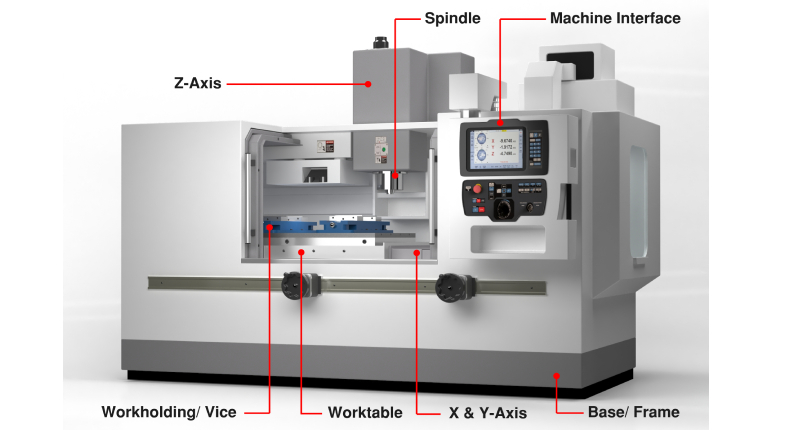
\includegraphics[scale=.6]{figures/basicCNC.jpg}}
	\caption{3-Axis CNC Machine \cite{3ax}}
	\label{3ax}
\end{figure}

Figure \ref{5ax} shows the schematic model of a 5-axis CNC machine. In this particular design, the spindle, which is responsible for cutting the workpiece, has the ability to move along three axes, namely the X, Y, and Z axes. This movement allows for precise control over the position and depth of the tool in relation to the workpiece.

In addition to the spindle movement, the machine features a rotary-tilt table that can adjust two additional axes, namely the A and B axes. These axes provide rotational and tilting capabilities to the worktable, allowing for more intricate movements and increased flexibility in part design. By adjusting the A and B axes, the workpiece can be positioned and oriented in different angles, enabling the CNC machine to access and machine complex geometries that would otherwise be difficult or impossible to achieve with fewer axes. Additionally, a tool magazine is included that allows for tool changes. In this way, a roughing and finishing operation can be performed without having to change the tool manually.

The inclusion of these two additional degrees of freedom in the 5-axis CNC machine significantly expands the range of operations that can be performed. It enables the machine to handle more complex and sophisticated machining tasks, such as multi-sided machining, contouring, and simultaneous machining on multiple surfaces. This increased flexibility and versatility make the 5-axis CNC machine a valuable tool in industries that require high precision and intricate part production.

\begin{figure}[H]
	\centerline{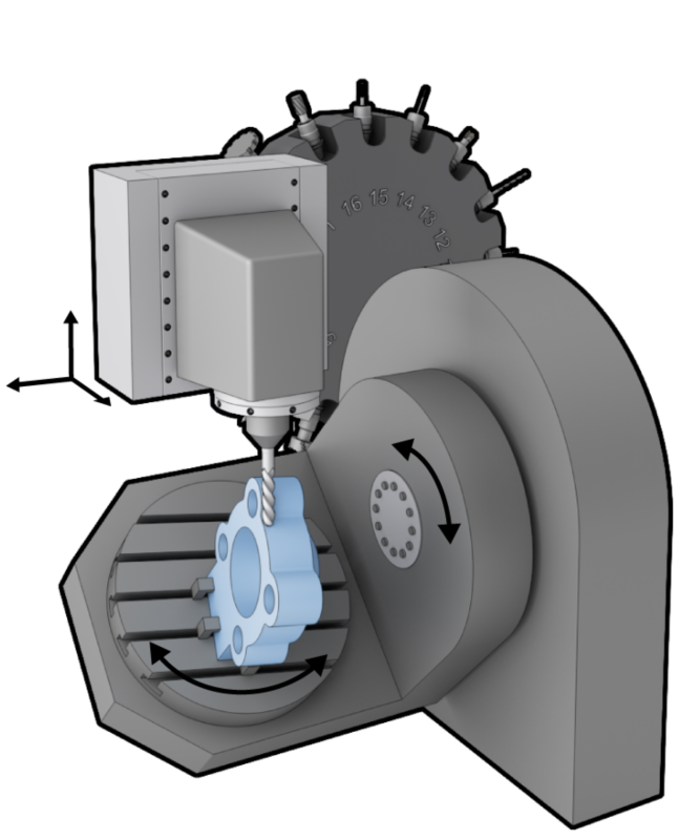
\includegraphics[scale=.45]{figures/5ax.png}}
	\caption{5-Axis CNC Machine \cite{5ax}}
	\label{5ax}
\end{figure}



\subsection{Additive Manufacturing}
AM processes involve the conversion of CAD files into physical objects by building them layer by layer. This layering approach offers several advantages. Firstly, it allows for the creation of complex geometries that would be extremely challenging or impossible to produce using traditional manufacturing methods~\cite{Prakash.2018}. The ability to fabricate intricate structures with internal cavities, undercuts, and overhangs opens up new possibilities in engineering and design~\cite{Abdulhameed.2019}.

Various AM technologies utilize different methods to build the layers. Fused Deposition Modeling (FDM), for example, involves extruding molten thermoplastic filament through a heated nozzle, which solidifies as it cools, creating the desired shape~\cite{Wickramasinghe.2020}. Stereolithography (SLA) employs a liquid photopolymer resin that is solidified by a UV laser, while Selective Laser Sintering (SLS) uses a high-power laser to selectively fuse powdered materials, such as plastics or metals~\cite{Wang.2016, Meier.2017}.

The compatibility of AM with a wide range of materials is another scientific advantage~\cite{Bose.2018}. It enables the production of components with diverse properties, including strength, flexibility, conductivity, and heat resistance. AM can accommodate various plastics, such as ABS, PLA, and nylon, as well as metals like titanium, aluminum, and stainless steel. Additionally, ceramics and even biomaterials, like hydrogels or living cells, can be used in AM processes. New materials specifically tailored for AM are continuously developed,  expanding the possibilities for unique applications~\cite{Attaran.2017}.

The design freedom offered by AM is a significant scientific breakthrough. Traditional manufacturing methods often have design constraints due to limitations in tooling and manufacturing processes. With AM, designers have greater flexibility to create complex and organic shapes, lightweight structures, and intricate internal features. This freedom leads to optimized performance and improved functionality~\cite{Plocher.2019}.

However, AM also poses scientific challenges. Post-processing requirements, such as smoothing, polishing, or heat treatment, may be necessary to achieve the desired surface finish or material properties~\cite{Jandyal.2022}. Additionally, certain applications may have limited material options, particularly in terms of high-temperature or high-strength applications. Production speed can also be a constraint for large or complex parts, as AM processes can be time-consuming compared to traditional manufacturing methods~\cite{Dilberoglu.2017}.

%AM has a significant impacts across various industries. In aerospace, AM is used to produce lightweight components, reducing fuel consumption and enhancing overall efficiency. In healthcare, AM has revolutionized medical device manufacturing, allowing for the production of patient-specific implants, prosthetics, and surgical guides. The automotive industry benefits from AM's ability to create complex and lightweight structures, improving vehicle performance and fuel economy. In the consumer goods sector, AM enables customization and personalization, allowing consumers to create unique and tailored products.

As AM technologies continue to advance, they have the potential to transform supply chains. The concept of distributed manufacturing, where products are produced closer to the point of use, becomes feasible with AM~\cite{Jandyal.2022}. This reduces transportation costs, lowers carbon emissions, and enables on-demand manufacturing, leading to shorter lead times and increased sustainability~\cite{Haleem.2019}.

%The high application rates, which range from 1 kg/h (aluminum and titanium) to 4 kg/h (steel), for example, make it possible to build large components at reasonable production times. Thus, most components can be produced within one working day. Compared to other additive manufacturing processes such as Powder Bed Fusion (PBF) with order collars of 0.1 - 0.36 kg/h (for Ti6Al4V), this can mean a time advantage with a factor of up to 10. In terms of part size, the maximum production volume is limited only by the working range of the kinematics used. In the case of an articulated-arm robot, this corresponds to the range within the minimum and maximum reach. The disadvantages of the WAAM are the residual stresses and deformations remaining after the process, the low geometric accuracy and the moderate surface quality. These problems are among the typical defects of WAAM components.

Figure \ref{3D} shows a commercially available 3D printer. The base plate has the ability to move along the Y axis, which allows for horizontal movement of the printed object. On the other hand, the print head can move along the X and Z axes. The X-axis movement controls the horizontal positioning of the print head, while the Z-axis movement controls the vertical positioning. This combination of movements in the X and Z axes enables the print head to accurately deposit layers of material to create the desired 3D object.

\begin{figure}[H]
	\centerline{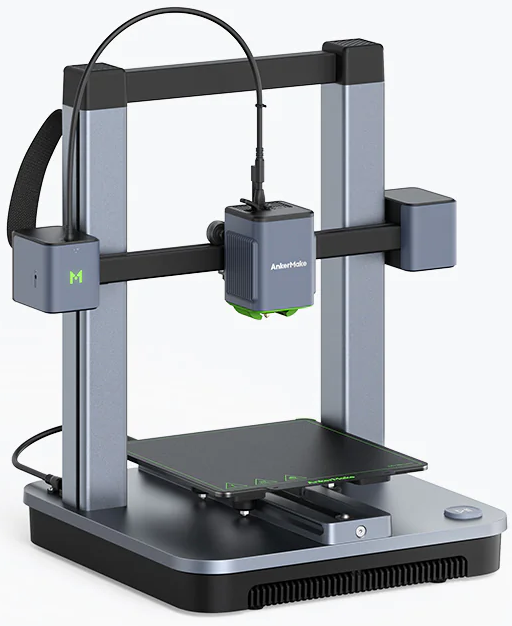
\includegraphics[scale=.5]{figures/3Dprinter.png}}
	\caption{3D Printer \cite{3D}}
	\label{3D}
\end{figure}

\subsubsection{Wire Arc Additive Manufacturing}
Wire Arc Additive Manufacturing (WAAM) is a specific type of additive manufacturing process known as Directed Energy Deposition (DED)~\cite{Svetlizky.2021}. According to the DIN EN ISO 52900 standard, DED involves using focused thermal energy to melt material during the application process to build up the individual layers~\cite{Additive}. In the case of WAAM, an electric arc is used to generate the necessary energy for melting. This process is utilizing standard welding technology, such as gas-shielded metal arc welding, in combination with precise spatial movement of the welding torch~\cite{Cunningham.2018}. This allows for the construction of components layer by layer.

WAAM offers several advantages over other additive manufacturing techniques. One major advantage is its high deposition rate, which ranges up to 6kg/h. This high deposition rate enables the construction of large components in a relatively short amount of time. Components can be produced within a single workday, providing a significant time advantage compared to techniques like Powder Bed Fusion (PBF), which typically operate at much slower deposition rates~\cite{IvanTabernero.2018}.

Another advantage of WAAM is its capability to construct large components without limitations on part size. The production volume is only constrained by the working range of the kinematics employed. For example, in the case of an articulated-arm robot, the range is defined by its maximum reach. This means that WAAM has the potential to create components of various sizes without compromising its effectiveness~\cite{Li.2019}.

However, it is important to note that WAAM components may have some inherent defects. These include residual stresses and deformations that persist after the production process, as well as relatively low geometric precision and modest surface quality. These limitations should be taken into consideration when utilizing WAAM for manufacturing purposes~\cite{Wu.2018}.

Figure \ref{WAAM} shows a schematic representation of a WAAM process. In this process, a wire feeder is utilized to supply a continuous stream of material. The wire is then subjected to high heat generated by an electric arc. The wire is melted and then deposited onto a substrate plate. The substrate plate serves as the foundation or base on which the material is built. As the molten wire is deposited, it solidifies and fuses with the previous layers, gradually building up the desired 3D object.

\begin{figure}[H]
	\centerline{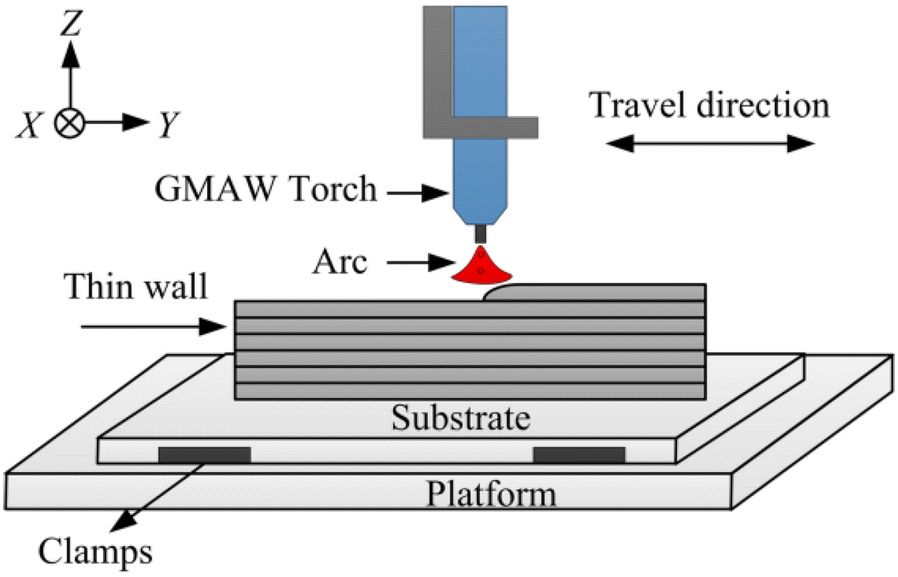
\includegraphics[scale=.12]{figures/WAAM.png}}
	\caption{Schematic representation of WAAM \cite{Jin.2020}}
	\label{WAAM}
\end{figure}

Figure \ref{WAAMba} shows a part produced by WAAM with the addition of a post processing step. The rough surface finish is clearly visible on the non post processed side of the part.

\begin{figure}[H]
	\centerline{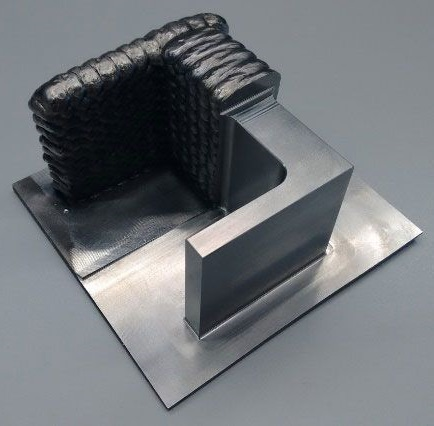
\includegraphics[scale=.8]{figures/WAAMba.jpg}}
	\caption{Part produced by WAAM with post machining \cite{WAAMba}}
	\label{WAAMba}
\end{figure}

\subsubsection{WAAM-Process and Cold Metal Transfer}
The operating principle of WAAM involves the generation of an arc through electrical discharge between an electrode and the workpiece. This arc transfers energy to the workpiece, causing melting in the fusion zone~\cite{Ou.2018}. Additionally, if a welding filler material in the form of a wire is introduced into the arc, it also melts and can be used to deposit additional material onto a metallic substrate~\cite{Cunningham.2018}. To ensure a continuous weld seam, a wire feed system can be employed~\cite{Ding.2015}.

The industrial manufacturing of components using WAAM involves a kinematic system that allows movement of the welding torch. This can be achieved using robot-configurations or gantry systems~\cite{Schmitz.2021}. Alternatively, a spatially fixed welding torch, combined with robotic kinematics or rotary-tilt table, can be used to move the component~\cite{Nagasai.2022}. %The WAAM process builds up the component layer by layer, following a predefined path.

Cold Metal Transfer (CMT) welding is a sophisticated process that merges the advantages of multiple welding techniques~\cite{Dutra.2015}. It functions based on the principle of controlled short-circuiting, wherein the welding torch generates a short circuit between the electrode and the workpiece. This short circuit triggers the melting of the tip of the wire and subsequent detachment. The detachment is assisted by a retraction of the wire. This process is generating a sequence of droplets that are transferred to the weld pool with remarkable precision~\cite{Selvi.2018, Srinivasan.2022}.

CMT welding provides superior heat control with lower heat input than conventional methods. The controlled arc and droplet transfer reduce the risk of overheating and distortion, making it suitable for thinner materials and heat-sensitive applications~\cite{Scotti.2020}. The process minimizes spatter formation, resulting in cleaner and smoother welds and reducing the requirement for post-weld cleaning~\cite{Srinivasan.2022}. %This process stands out for its exceptional weld quality. Its precise control over heat input and metal transfer results in improved fusion, reduced porosity, and an enhanced appearance of the weld bead.
CMT welding is ideal for applications that require the highest weld quality which includes structural fabrication and automotive manufacturing~\cite{Cong.2016}.

For dependable weld quality, CMT welding typically integrates advanced process control systems, which utilize adaptive control and real-time monitoring to consistently adjust welding parameters based on sensor feedback. This enhances the precision and dependability of the welding process~\cite{Pickin.2006}.

A CMT cycle consists of three phases~\cite{Selvi.2018}:\newline
1st - pulse phase: a high current pulse leads to the ignition of the arc, 
which melts the wire electrode. A droplet begins to form at the 
tip of the wire. The wire is moved forward in the direction of the 
workpiece.\newline
2nd - arc phase: The arc is kept burning at a lower current. 
burning at a lower current. This prevents the melt droplet from detaching early and 
from detaching prematurely and transferring to the workpiece.\newline
3d - short-circuit phase: as soon as the wire comes into contact with the substrate, 
the voltage drops to 0 V and the wire feeder is signaled to withdraw the wire. 
is signaled to withdraw the wire. This supports the droplet detachment 
from the wire into the molten bath.

Figure \ref{fig:CMT} shows the three Phases of a CMT cycle. The voltage is constant in the first two phases and drops to zero in the short circuit phase. The spike of current is clearly visible in the first phase which is also the shortest.

\begin{figure}[H]
	\centering
	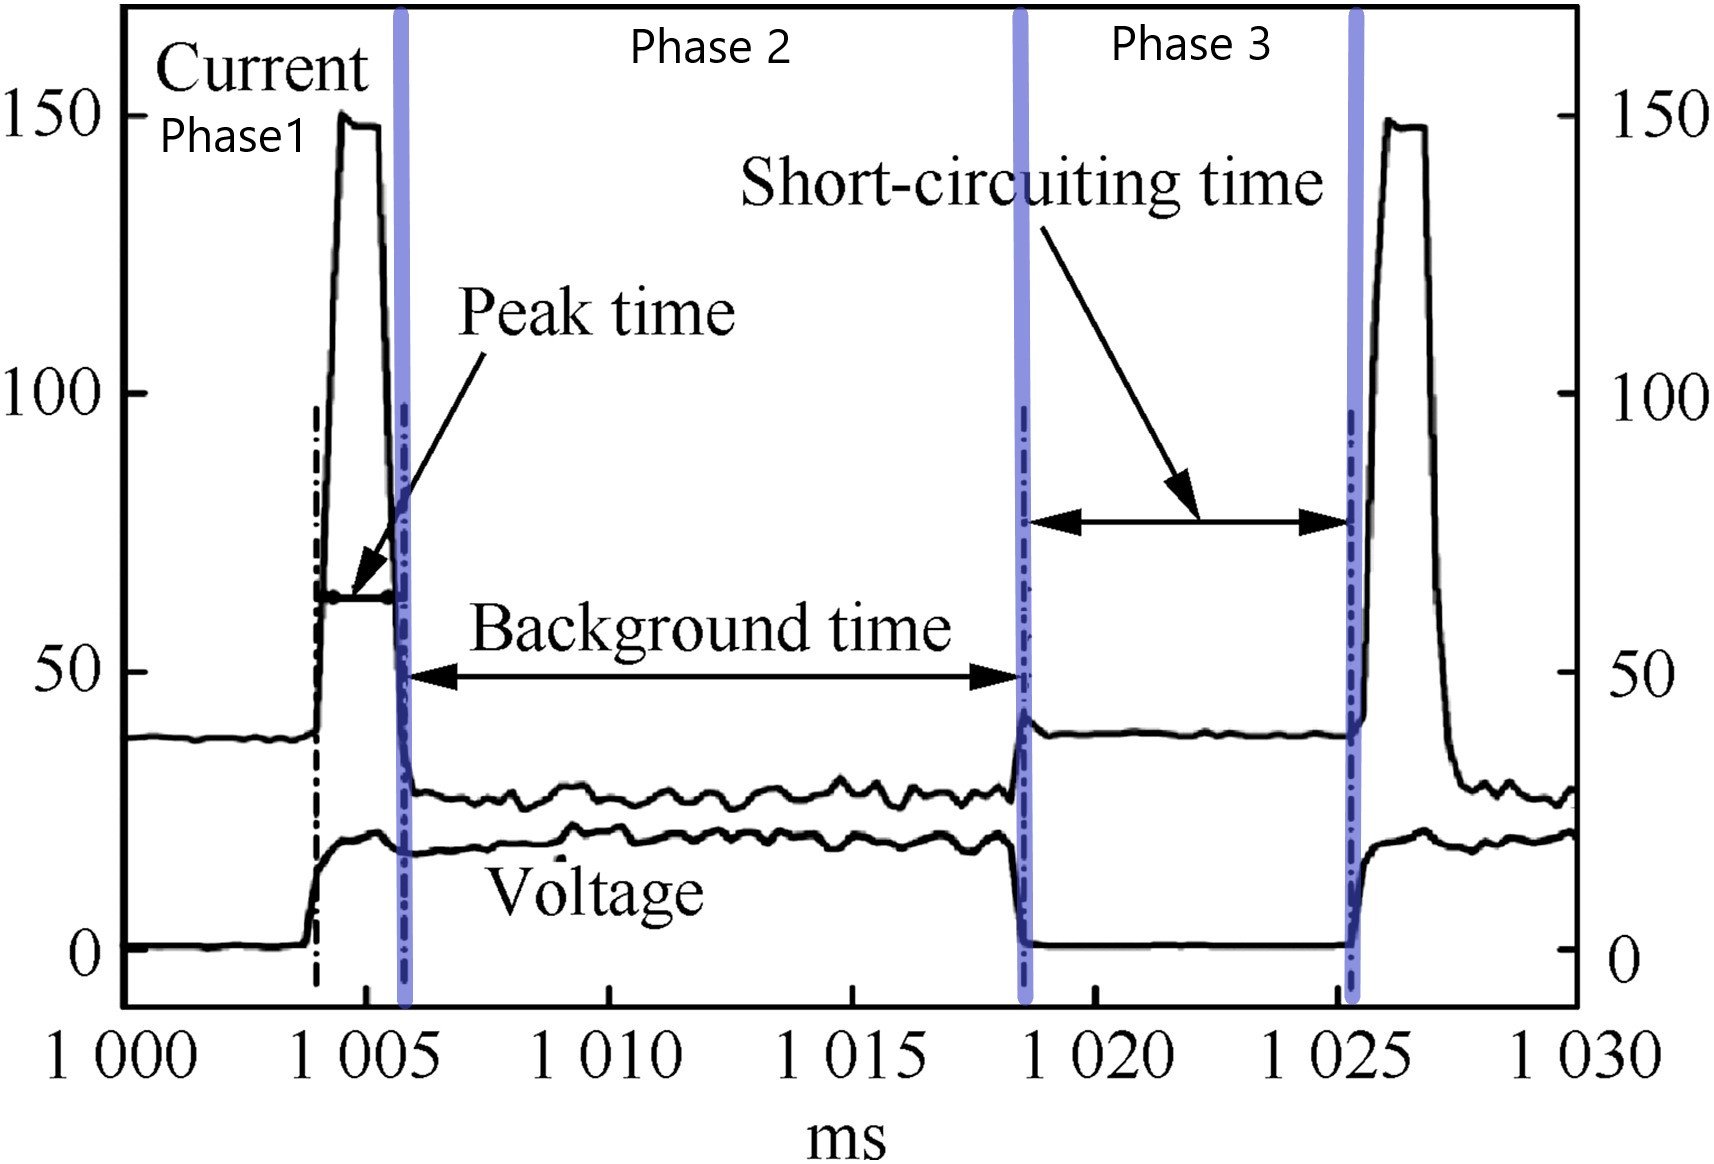
\includegraphics[width=0.6\linewidth]{figures/CMT.jpg}
	\caption{Current and Voltage wave forms of a CMT process~\cite{Selvi.2018}}
	\label{fig:CMT}
\end{figure}


Figure \ref{fig:CMT2} shows the clearly distinct parts in a CMT cycle. At first an electric arc is formed and melts the fire. After a short circuit is established the wire retracts and detaches from the molten droplet. After that the cycle restarts.

\begin{figure}[H]
	\centering
	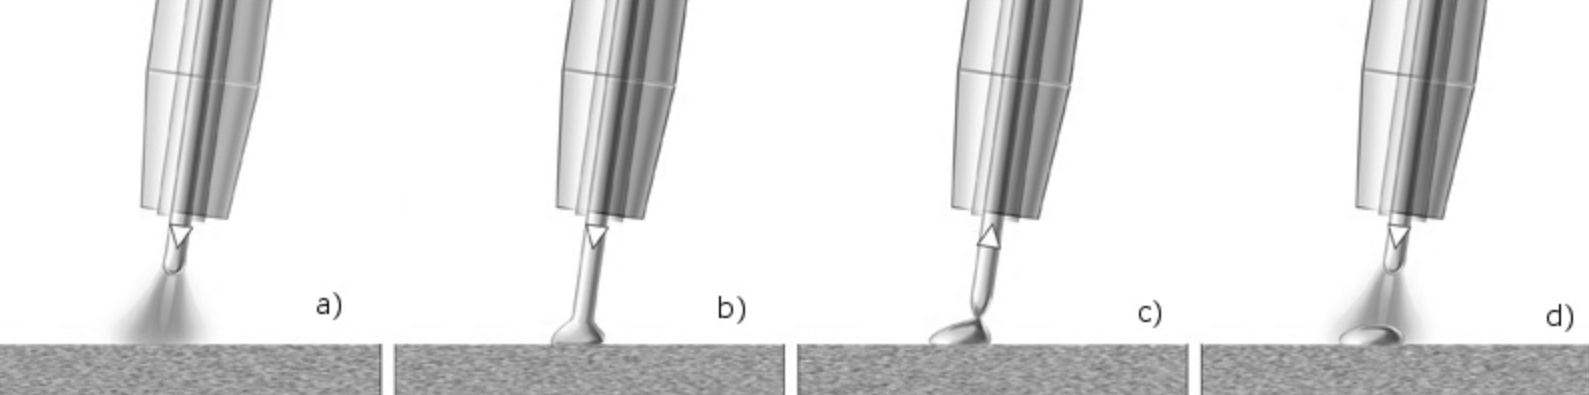
\includegraphics[width=0.9\linewidth]{figures/CMT2.png}
	\caption{Individual sections of a CMT cycle}
	\label{fig:CMT2}
\end{figure}


In summary, WAAM and CMT are highly sophisticated processes that enable the creation of 3D printed metal parts with specifically designed parameters. CMT achieves precise welds with low heat input and minimal spatter. It is ideal for thinner materials and applications requiring high weld quality. Advanced process control systems can enhance the reliability of CMT welding~\cite{Rahul.2018, Pickin.2011}.


%I FEEL SOMETHING IS MISSING !!!!\newline
%PLZ HELP\newline
%PLZ HELP\newline
%PLZ HELP\newline
%PLZ HELP\newline
%PLZ HELP


\subsection{Industrial Robots}\label{IR}
Industrial robots are advanced machines designed to perform various tasks in manufacturing and industrial settings. They come in different types, each with its own set of capabilities and advantages. They are crucial to modern manufacturing and automation, transforming production methods and repetitive task performance across diverse industries. Since their inception in the mid-20th century, these machines have undergone significant advancements, evolving into highly adaptive and sophisticated devices that promote productivity, accuracy, and safety within manufacturing processes~\cite{Ji.2019}.
At their core, industrial robots are programmable machines designed to execute tasks with a high degree of accuracy and efficiency. They can carry out repetitive actions consistently, which enhances productivity and reduces the risk of human error \cite{Siciliano.2016}. 



One common type of industrial robots are the articulated robots. These robots have rotary joints that allow them to move like a human arm, with multiple links and joints. They can perform a wide range of tasks, such as welding, material handling, or assembly operations~\cite{Hanafusa.1981, Jain.2019}. Another type is the Cartesian robot, also known as gantry robots. These robots move along three linear axes (X, Y, and Z) to perform tasks. They are commonly used for pick-and-place operations or in applications that require precise positioning~\cite{Kim.2003}. SCARA robots, on the other hand, are designed for fast and precise movements in assembly operations. They have a selective compliance assembly robot arm that allows them to move quickly while maintaining accuracy~\cite{Das.2005}. Delta robots are used for high-speed pick and place applications, such as packaging or sorting. They are known for their rapid movements and high throughput~\cite{bonev2001delta}. Collaborative robots, or cobots, are designed to work safely alongside humans. They have built-in safety features, such as force sensors or vision systems, that allow them to interact with humans without causing harm. Cobots are often used in tasks that require human-robot collaboration, such as assembly or inspection operations~\cite{Liu.2022b}.


Figure \ref{fig:ScaraDelta} shows a SCARA and Delta Robot.
\begin{figure}[H]%
	\centering
	\subfloat{{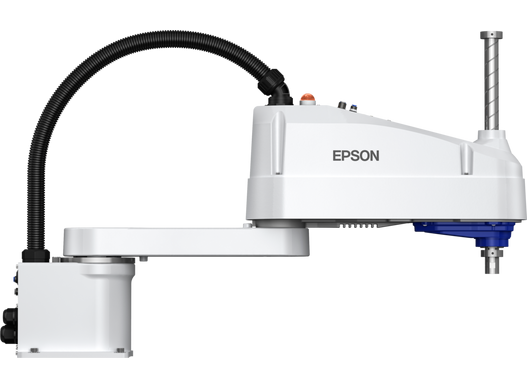
\includegraphics[width=5cm]{figures/scara.png} }}%
	\qquad
	\subfloat{{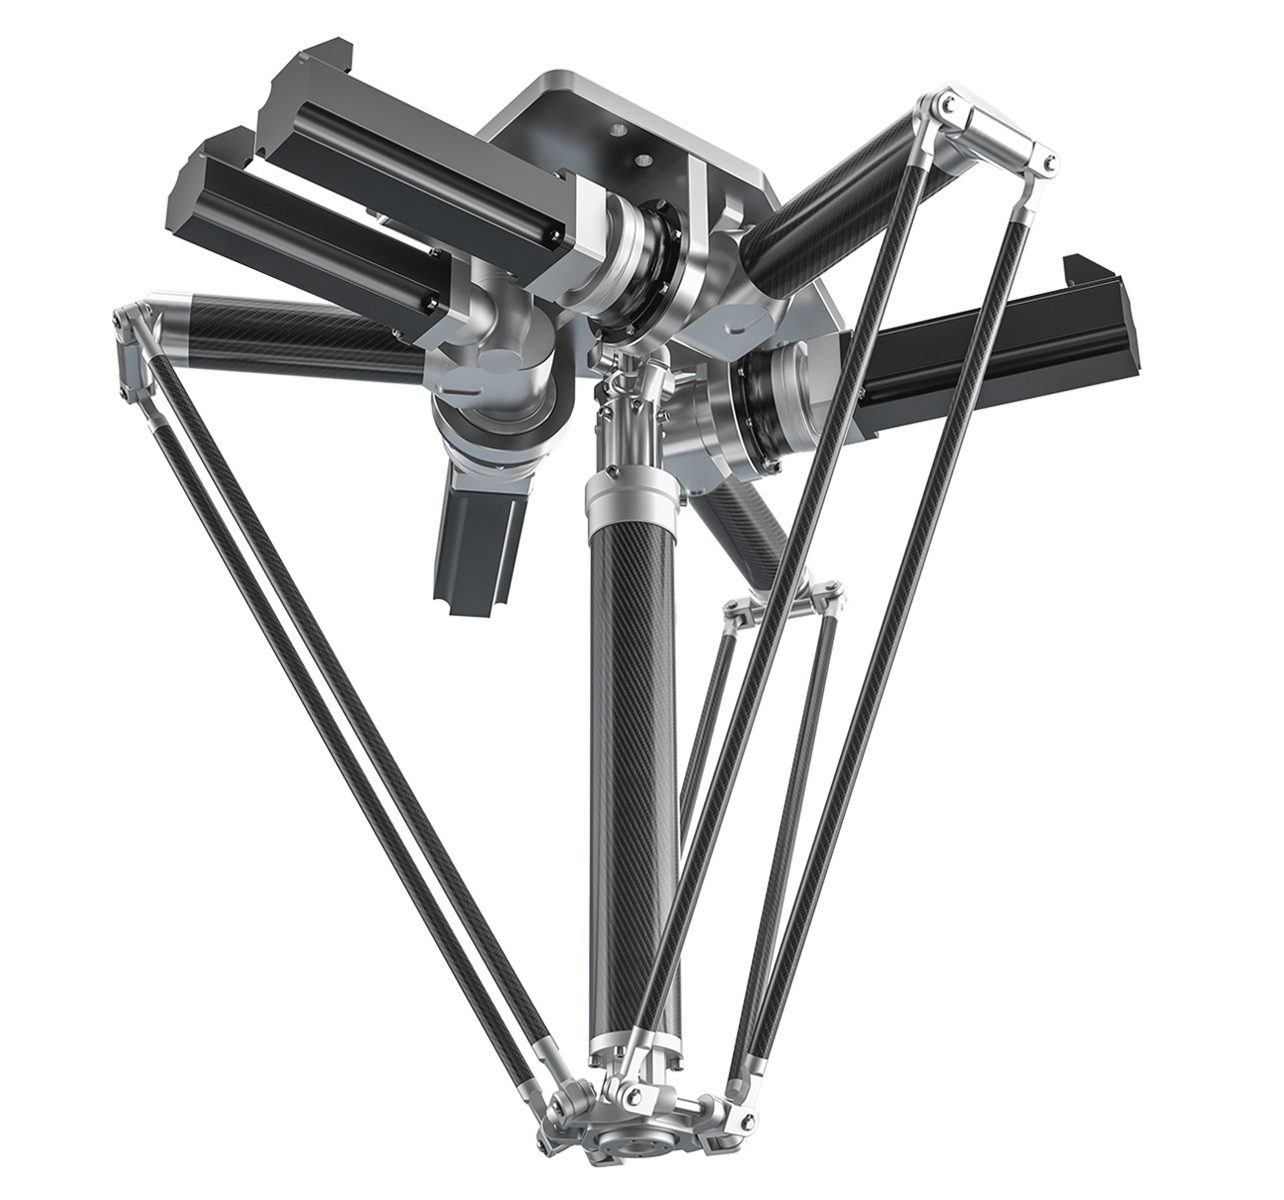
\includegraphics[width=5cm]{figures/delta.png} }}%
	\caption{SCARA and Delta Robot}%
	\label{fig:ScaraDelta}%
\end{figure}

Industrial robots are based on articulated robots and have a wide range of applications across various industries. They can be used for assembly operations, where they can perform tasks like fastening, welding, or soldering components together. These robots are also commonly used for material handling tasks, such as lifting, moving, and stacking materials in warehouses or production lines. Inspection tasks can be automated with robots equipped with sensors or cameras, allowing them to inspect products for defects or perform quality control checks \cite{Hagele.2016}.


Industrial robots offer several benefits. Firstly, they increase productivity by working continuously, without breaks or fatigue. This leads to higher production rates and shorter cycle times. Additionally, robots can perform tasks with high precision and accuracy, reducing errors and defects and thereby improving product quality \cite{Kubela.2016}. Safety is another important aspect of industrial robots. They are designed to handle dangerous or hazardous tasks, keeping human workers safe. Robots can work in environments with high temperatures, toxic substances, or heavy loads, minimizing the risk of injury to humans \cite{Heyer.2010}.
While the initial investment in industrial robots can be high, they offer long-term cost savings. Robots can reduce labor costs by automating repetitive tasks and increasing efficiency. They also offer flexibility, as they can be reprogrammed or reconfigured to perform different tasks, allowing for greater adaptability in manufacturing processes \cite{Jung.2020b}.

When comparing industrial robots to CNC machines, there are a few notable disadvantages for industrial robots. Firstly, industrial robots generally have lower positional accuracy and repeatability compared to CNC machines. CNC machines are purpose-built for precise machining operations and can achieve high levels of accuracy and repeatability \cite{Wang.2023}.
Secondly, industrial robots typically have a longer cycle time compared to CNC machines for similar tasks. The complex movements and computations involved in robot control can result in slower overall operation speeds, which may not be ideal for high-volume production environments \cite{Joshi.2021}.
Additionally, industrial robots can be more complex to program and set up than CNC machines. CNC machines follow a predefined set of instructions, whereas programming industrial robots often requires more advanced programming skills and can be time-consuming \cite{Ye.2022}. Lastly, industrial robots may have limitations when it comes to handling heavy loads or performing heavy-duty machining operations. CNC machines are specifically designed for heavy-duty cutting, milling, and drilling tasks, whereas industrial robots are better suited for lighter material handling and assembly operations \cite{Wu.2022}. These differences should be considered when deciding between industrial robots and CNC machines for specific manufacturing applications.

Industrial robots can be programmed using different methods. One common method is using a teach pendant, where operators manually move the robot to record positions and actions. Offline programming is another approach, where programs are created and simulated on a computer before being transferred to the robot. Sensor-based programming allows robots to respond to sensor inputs or interact with the environment \cite{Heimann.2020}. %More information regarding the control of robots is described in Chapter \ref{CAMmain}.


Serial kinematics is a widely used configuration in industrial robots, where the robot arm is constructed as a sequential chain of joints and links. Each joint provides one DoF, enabling the robot to move and position its end-effector in a controlled manner. The joints can be of various types, including revolute, prismatic, spherical, and cylindrical, providing rotational, linear, and combined movements. The motion of the robot arm is controlled using forward kinematics and inverse kinematics. Forward kinematics calculates the position and orientation of the end-effector based on the joint angles, while inverse kinematics determines the joint angles required to achieve the desired end-effector pose \cite{Singh.2021b}. %Serial kinematics robots have significantly contributed to automation processes, enhancing productivity, efficiency, and flexibility in manufacturing industries.


In summary, the robots performance relies on sophisticated control algorithms and feedback systems that allow them to adapt to dynamic conditions, adjust movements in real-time, and maintain a consistently high level of accuracy \cite{Lin.2023}. This improves both the quality of the final product and the safety of the manufacturing process, as robots can navigate complex paths without risking collisions or accidents~\cite{Bosscher.2011}.
As technology continues to advance, industrial robots will play an even more prominent role in shaping the future of manufacturing and automation \cite{Domae.2019}


Figure \ref{robot} shows the schematic design of a 6-DoF industrial robot with a spindle and force sensor that is used for machining.

\begin{figure}[H]
	\centerline{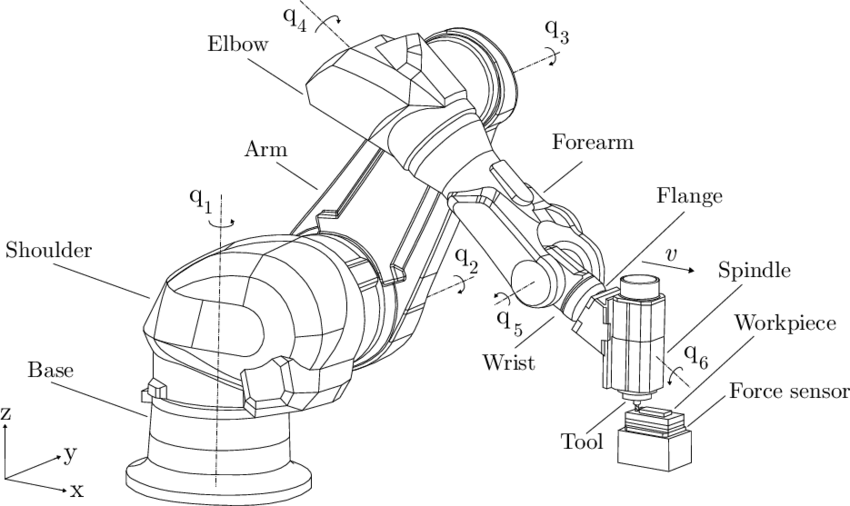
\includegraphics[scale=.4]{figures/robot.png}}
	\caption{6-DoF industrial Robot \cite{HuynhHoaiNam.2018}}
	\label{robot}
\end{figure}


\subsubsection{Redundancy in robotic systems}

Industrial robots with redundant degrees of freedom are robotic systems that have been designed with more degrees of freedom (DOF) than are necessary for a specific task \cite{Liu.2022}. This extra DOF allows the robots to perform additional joint movements or configurations beyond what is required for basic movement or manipulation.

The primary advantage of these redundant robots is their increased flexibility and adaptability \cite{Duong.2021}. Robots with more DOF can access a wider range of positions and orientations, making it possible for them to complete complex tasks in constrained environments that would have been difficult or impossible otherwise. With this added flexibility, they can avoid obstacles and work around them without disrupting their duties. In industrial settings, redundant manipulators provide significant advantages. Their additional degrees of freedom enable them to improve accessibility to hard-to-reach areas and enhance overall operational capabilities \cite{Shi.2021}.   

Redundancy can take on many different forms in robotic systems. One option is to increase the number of joints in the serial kinematics of an articulated robot \cite{Milenkovic.2021}. Another approach to redundancy is the addition of a rotary tilt table, which is commonly used in WAAM in combination with a 6-DoF robot \cite{Yuan.2020}. This combined system enables the robot to manipulate the workpiece from various angles, enhancing the manufacturing process.

Furthermore, the inclusion of a linear axis that the robot base can traverse on is yet another form of redundant DoF. This additional linear motion provides the robot with extended reach and the capability to access a larger workspace, making it suitable for tasks that require movement along a specific axis \cite{Boscariol.2019}.

Additionally, redundancy can also be observed when using a generic 6-DoF system for operations that only necessitate 5 or fewer DoF (for example, milling or WAAM) \cite{Hanafusa.1981,Liu.2022}. The system possesses more flexibility than required for the specific task and allows for adaptability and versatility, thus accommodating different operations without the need for reconfiguring the robot.

In summary, redundancy in robotic systems can be achieved through various means, such as increasing joint numbers, incorporating rotary tilt tables, including linear axes, or using a higher DoF system for tasks that demand fewer DoF. These redundant features enhance the capabilities and versatility of the robot, enabling it to perform a wide range of complex tasks efficiently.

Figure \ref{linear} shows two industrial robots from the manufacturer KUKA GmbH that are placed on a linear axis. This enables the robots to use the additional and redundant DoF to optimize the process. Multiple robots can be positioned on one linear unit. 
Figure \ref{seven} shows how a 7-DoF robot can have multiple poses reaching the same position. In this case, only six DoF are necessary to achieve the position, while one DoF can be defined manually.

\begin{figure}[H]
	\centerline{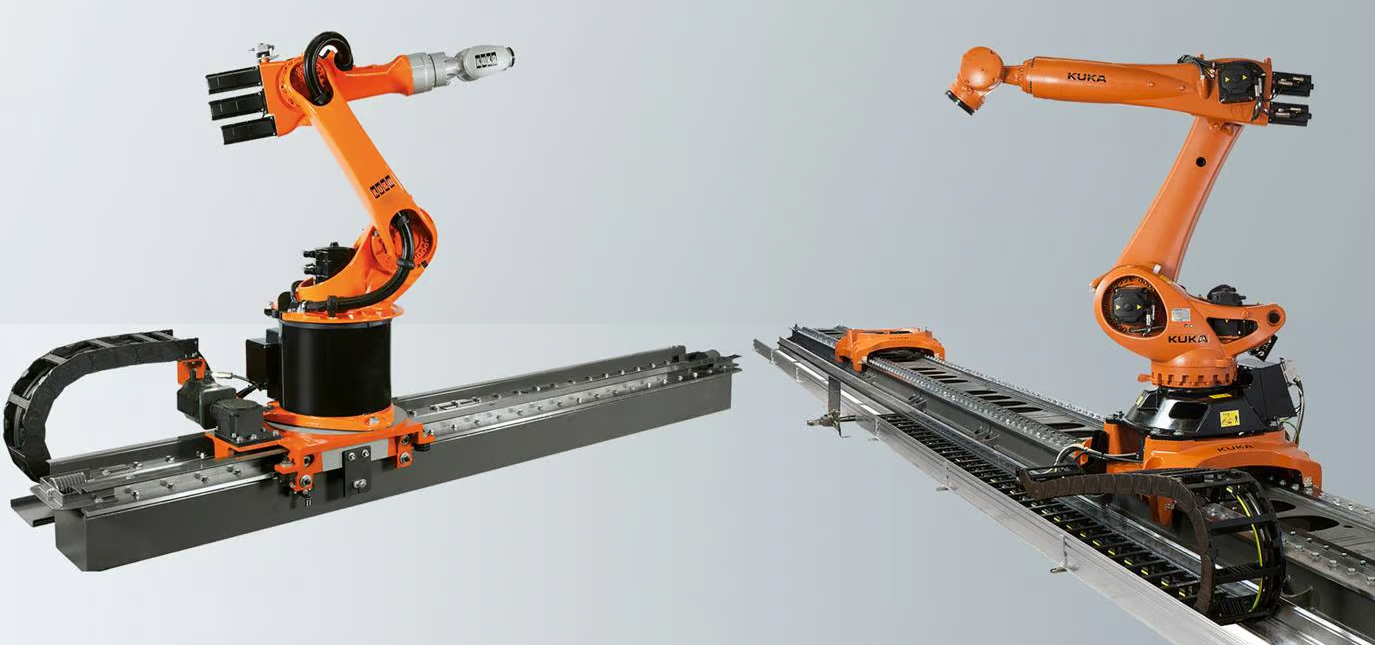
\includegraphics[scale=.4]{figures/linear.png}}
	\caption{Industrial robots with an additional linear axis \cite{linear}}
	\label{linear}
\end{figure}

\begin{figure}[H]
	\centerline{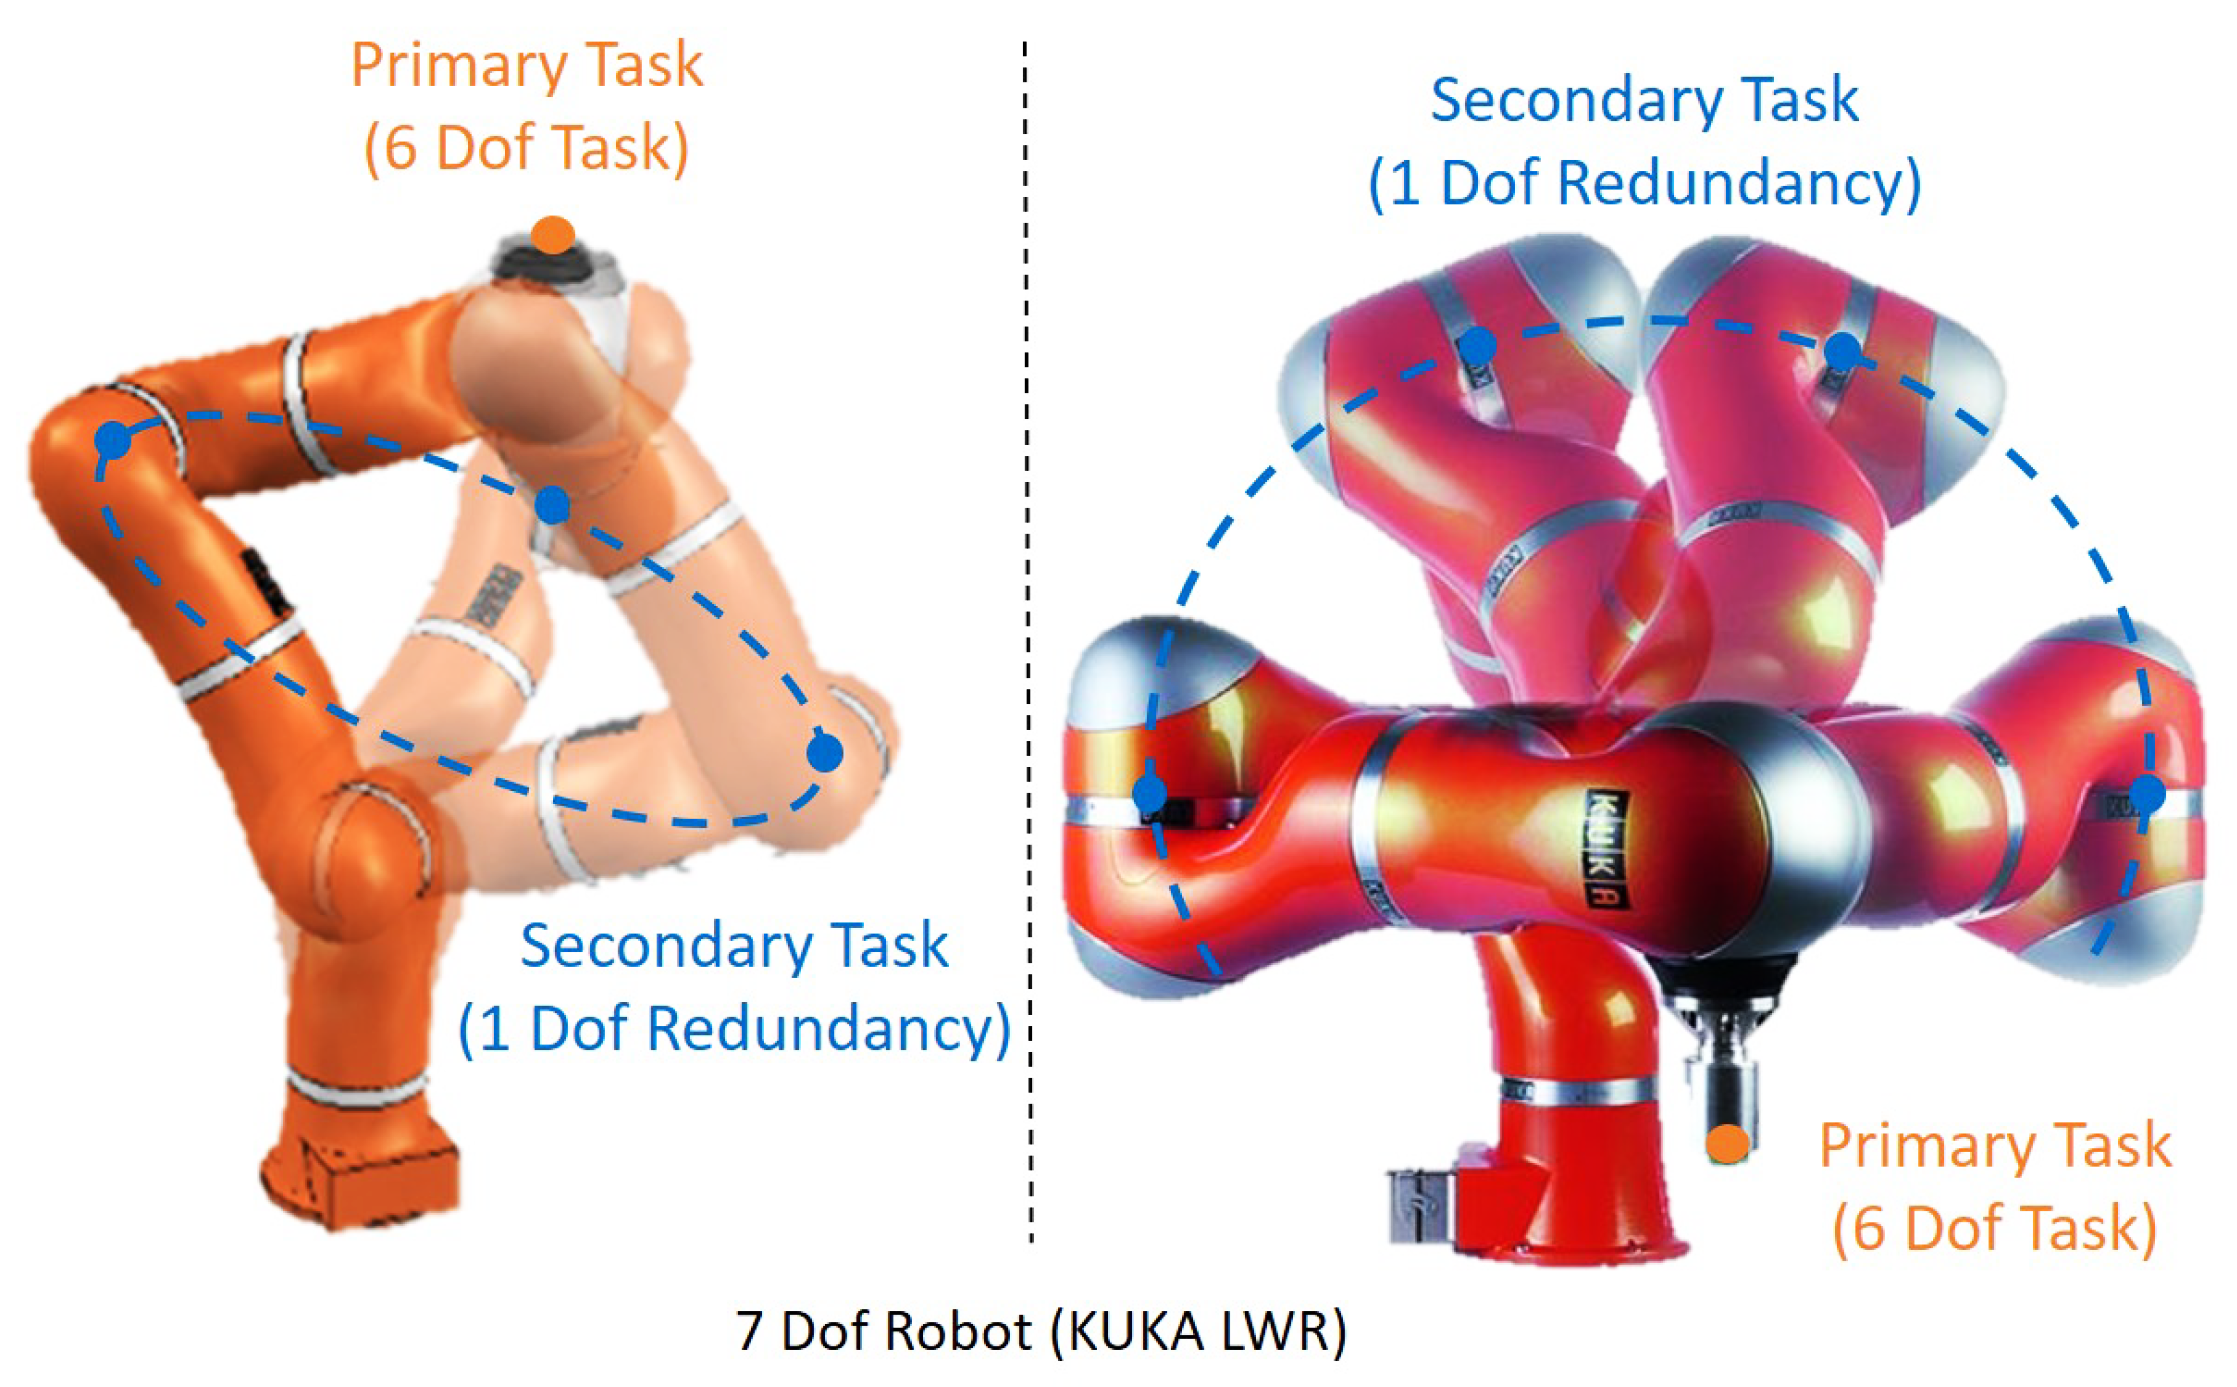
\includegraphics[scale=.14]{figures/red.png}}
	\caption{7 DoF robot \cite{Hagane.2022}}
	\label{seven}
\end{figure}



While redundancy in industrial robots can provide increased flexibility and adaptability, it also comes with certain disadvantages. One major drawback is the increased complexity and cost associated with redundant systems \cite{Halevi.2011}. The addition of extra joints, axes, or mechanisms adds to the overall complexity of the robot, requiring more sophisticated control algorithms and hardware \cite{Duong.2021}. This complexity not only increases the initial cost of the robot but also adds to the maintenance and troubleshooting efforts \cite{Ahangar.2019}. Additionally, the presence of redundant DoF can make the robot more susceptible to mechanical failures as more components are involved. This can result in increased downtime and higher maintenance costs. Moreover, the increased complexity of redundant systems can make programming and calibration more challenging, requiring specialized skills and expertise \cite{Erdos.2016}. Therefore, while redundancy can offer advantages in certain scenarios, careful consideration must be given to the cost, complexity, and maintenance implications before implementing it in industrial robotics applications.




\subsubsection{Continuous-path mode}
In the context of industrial robotics, continuous paths without abrupt direction or velocity changes of a tool play a crucial role in achieving precise and smooth movements of robotic arms along a defined trajectory \cite{Jia.2018}. This ensures that the robot can execute complex tasks and movements with accuracy and efficiency. By incorporating continuous path mode into industrial robot programming, manufacturers can optimize production processes and improve the quality of manufactured products \cite{Zhang.2020}. Constant velocity of a tool is especially important in applications like WAAM where the quality of the layer is directly dependent on the federate \cite{Li.2018b}. In CNC machining, discontinuities in velocity, acceleration, and jerk result in non-optimal surface finishes \cite{Sun.2021}.


Continuous path mode refers to a mode of operation in high-speed robotics as well as CNC machines where the goal is to achieve a smooth and uninterrupted movement of the machine along a toolpath. In this mode, the machine is expected to follow a path without any sudden changes in velocity, acceleration, or curvature. The purpose of continuous path mode is to minimize jerk spikes, machine vibrations, and other undesirable effects that can occur when there are discontinuities in the toolpath \cite{Jia.2018, Yang.2017}.

Figure \ref{C1} shows where the smooth-path-requirement comes into conflict with the tool path, which is based on the part geometry. Sharp corners and small radii can require significant acceleration to maintain a constant velocity. 


 \begin{figure}[H]
 	\centerline{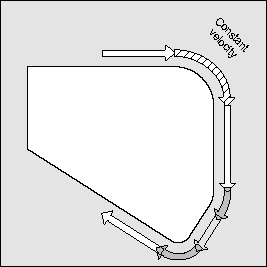
\includegraphics[scale=.25]{figures/conti.png}}
 	\caption{Desired path with constant velocity \cite{sinumericmanual}}
 	\label{C1}
 \end{figure}
 
Figure \ref{C2} shows how specific G-code commands of the SINUMERIK 840D influence the targeted feedrate. When using the G60 command, the points are reached exactly, but the feedrate is reducing to 0 at every waypoint. When implementing the G64 command, the feedrate can be held at the desired value.
 
 \begin{figure}[H]
 	\centerline{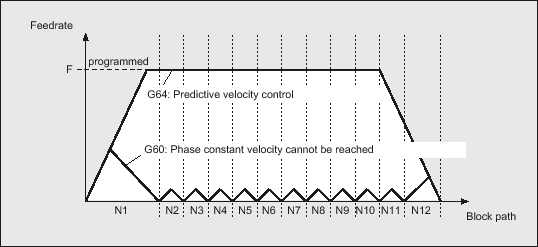
\includegraphics[scale=0.25]{figures/conti1.png}}
 	\caption{Influence of G-Code commands regarding feedrate compliance \cite{sinumericmanual}}
 	\label{C2}
 \end{figure}
 
Figure \ref{C3} shows how the G-code command G641 ADIS=0.5 of the SINUMERIK 840D is influencing the programmed contour. The rounding of the path begins no more than 0.5 mm before the programmed end of the block and must finish 0.5 mm after the end of the block. 
 
 \begin{figure}[H]
 	\centerline{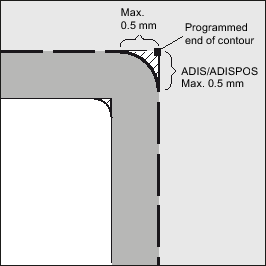
\includegraphics[scale=.25]{figures/conti2.png}}
 	\caption{Predetermined deviation of the programmed and executed path \cite{sinumericmanual}}
 	\label{C3}
 \end{figure}

Figure \ref{C4} shows how commands G601 and 602 influence the executed trajectory. In this case, two different tolerance limits allow the tool to deviate from the programmed path.
 
  \begin{figure}[H]
 	\centerline{\includegraphics[scale=.25]{figures/conti3.png}}
 	\caption{Influence of commands G601 and G602 \cite{sinumericmanual}}
 	\label{C4}
 \end{figure}
 
 
 
Continuous-path mode in CNC machining is a crucial aspect when it comes to processing parts with rapidly varied geometric features. These types of components, often found in high-end equipment, pose challenges due to their intricate structures and strict requirements. The presence of rapidly varied geometric features, coupled with the continuous-path running characteristic, gives rise to trajectory errors during the machining process, which severely hampers the overall machining accuracy of such parts \cite{Shahzadeh.2018}. This becomes even more critical in high-feed-speed machining scenarios, where existing studies struggle to effectively reduce this error without compromising machining efficiency \cite{Li.2018}.

In CNC machines, toolpaths are typically composed of lines and arcs \cite{Liu.2020}. At the transition points between these elements, careful consideration is required to ensure that the physical limits of the machine are not exceeded. For example, when the machine is moving at a constant feedrate, a sudden change in velocity can occur when two successive non-tangent linear moves meet. This can lead to undesirable effects on the machine and the quality of the cut \cite{Boujelbene.2004}. Similar issues arise at transitions between lines and arcs or between two arcs, where curvature discontinuities need to be addressed.  

Contouring errors are caused by factors such as servo lag, dynamics mismatch, external disturbances, and more. Reducing contouring errors is essential for improving the performance of CNC motion systems and achieving high-speed and high-precision machining \cite{Jia.2018}. 

To overcome these challenges and achieve a smooth and continuous toolpath, path smoothing techniques are necessary. Many path smoothing methods have been proposed in the literature, but most of them are limited to linear toolpaths. However, in high-speed CNC machines and industrial robots, the toolpaths often consist of both lines and arcs. Therefore, there is a need for a path smoothing method that can handle both line-to-line transitions and transitions involving arcs \cite{Shahzadeh.2018}.  


To address this issue and enhance both processing efficiency and precision, various estimation and compensation methods have been proposed for reducing trajectory error. These approaches can be divided into contouring-error estimation and contouring-error reduction approaches \cite{Jia.2018}. These approaches include the "Moving frame based method", "Analytical method", "Generalized method" or "Servo-tuning
approach". While this review paper compares the representative algorithms commonly used for contouring-error estimation and reduction, it is important to note that the comparison results only offer relative significance. Each algorithm has its own optimal range of applications and may outperform other methods within that range. Additionally, it is important to note that not every approach can be implemented on every system.


%The actual reachable feed speed is determined based on the geometry and drive constraints of the CNC machine tool.

%The continuous-path running trajectory error is estimated by approximating the desired toolpath using spline curves. Furthermore, a combination of mirror compensation and Taylor's expansion compensation can be employed as an error compensation approach \cite{Jia.2018}.

%One notable advantage of this proposed approach is its ease of estimation and compensation for continuous-path running trajectory errors by analyzing and modifying the NC codes. This implies a high level of feasibility for free-form toolpaths. Experimental results have demonstrated the favorable performance and effectiveness of these methods. By reducing the trajectory error in multi-axis high-speed machining, this study offers an effective approach to enhance the machining precision and efficiency of parts with rapidly varied geometric features in engineering applications. \cite{Song.2017}


Another approach for achieving continuous path mode is by using biclothoid fillets. These fillets are used for corner smoothing and can be fitted between two arcs or a line and an arc. The main advantage of using biclothoid fillets is that they result in a smoother curvature profile compared to other methods, such as Bezier fillets. Especially with tight tolerance values, only a few biclothoid fillets are needed compared to Bezier fillets. Additionally, the biclothoid approach is more suitable in regards to the jerk and acceleration limits of the driving units. This smoother curvature profile allows for higher feedrates and shorter cycle times, ultimately improving the overall performance of the CNC machine \cite{Shahzadeh.2018}.  







%MORE SINUMERIC HERE \cite{sinumericmanual} ?????????
%gemeinsamkeitmnen \newline
%prozesskräfte \newline
%was ist wichtig bei fräsen unf WAAM \newline 
\newpage
\section{Computer-Aided Manufacturing}\label{CAMmain}

CAM is a technology that uses computer software to automate and optimize manufacturing processes. It involves the use of computer systems to control and operate machinery, such as CNC machines, robots, and 3D printers. CAM software can generate tool paths and instructions for machines based on Computer-Aided Design (CAD) models, allowing for precise and efficient production. By reducing manual labor, CAM helps improve productivity, accuracy, and consistency in manufacturing. It is widely used in industries like aerospace, automotive, and electronics to streamline production and reduce costs \cite{Bi.2021}.

\subsection{CAM Software}

CAM software is a type of computer software used to automate and optimize the manufacturing process. CAM software takes the design data from computer-aided design (CAD) software and converts it into instructions that control machines and tools to produce the desired product \cite{Bi.2021}. It plays a critical role in modern manufacturing, helping to streamline production, improve efficiency, and reduce errors.

CAM software enables manufacturers to generate toolpaths and machining instructions for a variety of manufacturing processes, including milling, turning, drilling, and 3D printing \cite{Kumar.2019}. It takes into account factors such as material properties, tool capabilities, and manufacturing constraints to generate the most efficient and accurate instructions for the machines. CAM software can also simulate the machining process to detect any potential collisions or issues before actual production begins, saving time and resources \cite{Bui.2019}.

One of the key features of CAM software is its ability to optimize the machining process. It can automatically optimize toolpaths to minimize machining time, reduce material waste, and improve surface finish. By analyzing the geometry of the part, the software can determine the most efficient toolpath strategies, such as contouring, pocketing, or adaptive machining. It can also optimize tool selection, toolpath sequencing, and cutting parameters to achieve the best possible results \cite{Kyratsis.2020}.

It also offers advanced features such as multi-axis machining and support for complex geometries. It can generate toolpaths for machines with multiple axes of motion, allowing for more intricate and precise machining operations. It can handle complex geometries, including freeform surfaces and curved profiles, and generate toolpaths that accurately follow the desired shape \cite{Liang.2021}.

Furthermore, CAM software often integrates with other manufacturing software systems, such as computer-aided engineering (CAE) and enterprise resource planning (ERP) systems \cite{Ramazanov.2020}. This integration enables seamless data exchange, improves collaboration between different departments, and ensures that the manufacturing process is aligned with the overall production goals \cite{Kadam.2023}.

CAM software is a crucial tool for modern manufacturing. It automates and optimizes the manufacturing process, generating toolpaths and machining instructions based on CAD data. It enables manufacturers to improve efficiency, reduce errors, and achieve higher-quality products. With features such as optimization, simulation, multi-axis machining, and integration with other systems, CAM software empowers manufacturers to stay competitive in today's fast-paced and complex manufacturing environment \cite{Kappmeyer.2021}.

Figure \ref{CAMinterface} shows the interface of Siemens NX, a CAM/CAD software that can be used to design parts and generate machine-specific instructions for manufacturing. 

\begin{figure}[H]
	\centerline{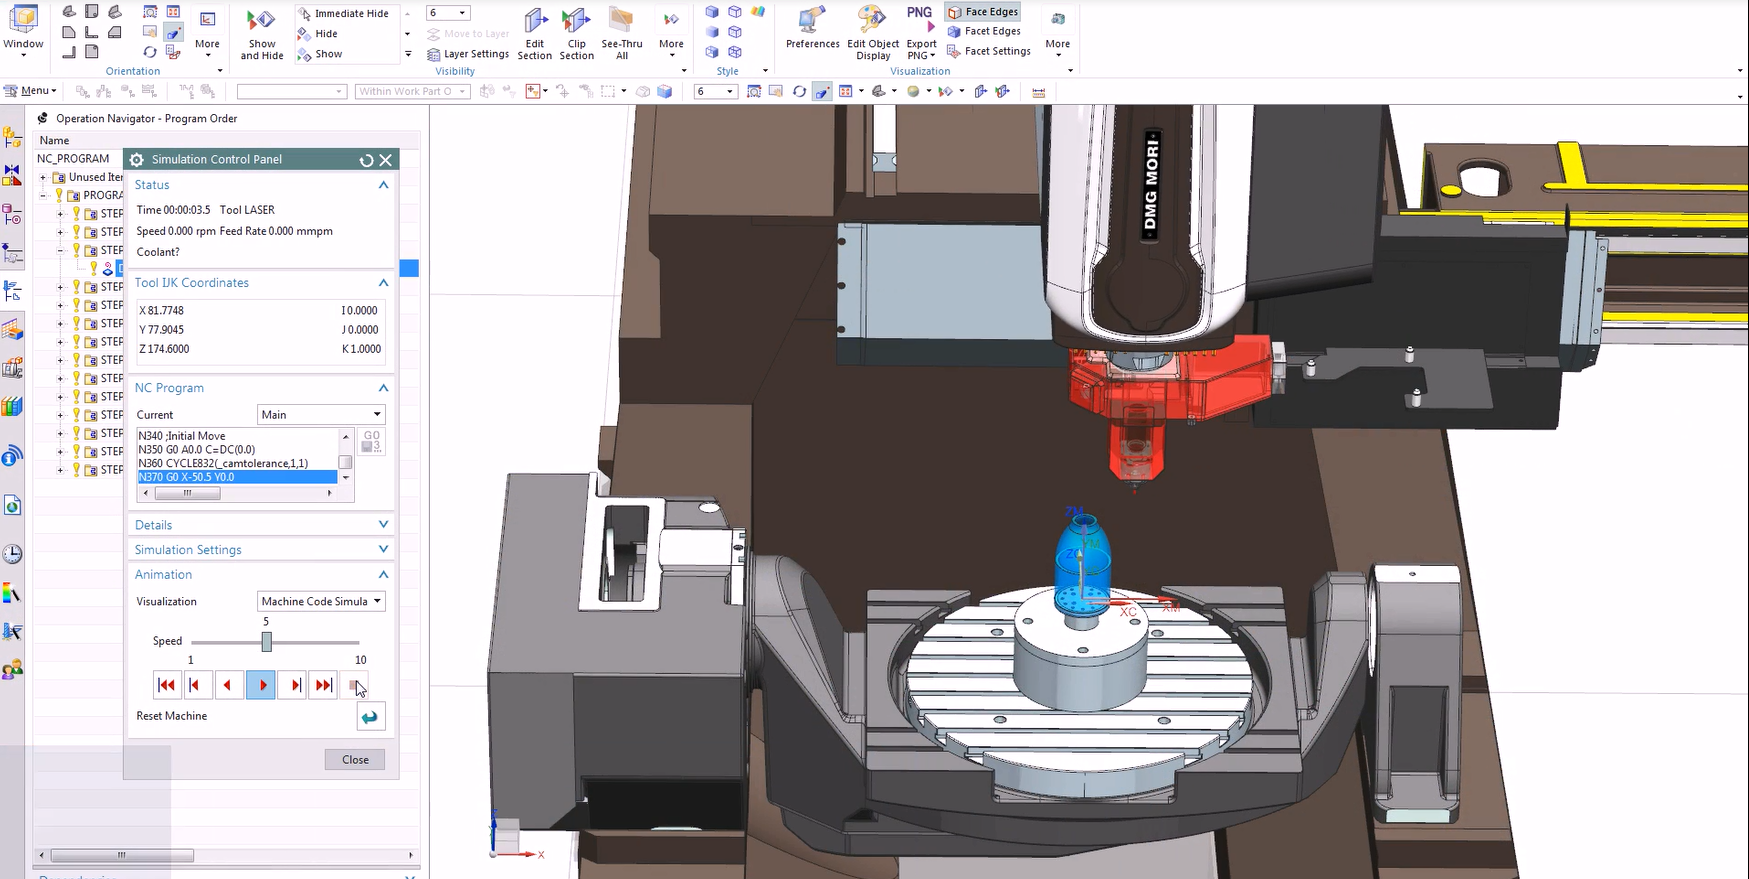
\includegraphics[scale=.4]{figures/CAM.png}}
	\caption{Interface of Siemens NX \cite{NXManufacturing.2015}}
	\label{CAMinterface}
\end{figure}


\subsection{Path Planning}
Path planning and generation are crucial features of CAM software. They involve establishing the most effective toolpaths for machining operations, guaranteeing efficient and precise production \cite{Brecher.2013}.

Path planning involves determining the optimal sequence of movements for the machining tool to follow while producing a component. It considers factors such as part geometry, tool capabilities, machining constraints, and desired parameters. Its goal is to minimize machining time, reduce waste, and improve the finished product \cite{Xu.2015}.  CAM software employs algorithms and mathematical models to determine the tool's position and orientation on the toolpath. Additionally, factors such as cutting direction, feed rate, and tool engagement need to be taken into account\cite{Tunc.2017}.

Adaptive machining is a critical part of path planning and generation. It enables the CAM software to adjust the toolpath and cutting parameters in real-time based on material properties, tool wear, and other factors. This constant monitoring and adaptation ensure precise and dependable outcomes, even in difficult manufacturing conditions \cite{Liu.2017}.

Multi-axis machining is an advanced function of CAM software, ideal for intricate cuts and shapes on complex geometries. By allowing the tool to move simultaneously along multiple axes, it delivers greater precision and accuracy during the machining of curved surfaces, freeform shapes, or parts with undercuts \cite{Takeuchi.2014}.

Simulation is vital in planning and generating paths for this process. CAM software typically includes simulation tools that enable users to visualize and verify the toolpath prior to production. These simulations can detect and resolve potential collisions, interference, or errors that may occur during machining, leading to cost savings and increased safety \cite{Dubovska.2014}. 

Figure \ref{3path} shows three different path trajectories for planar milling operations. Depending on the area of application, different paths can be optimal.  

\begin{figure}[H]
	\centerline{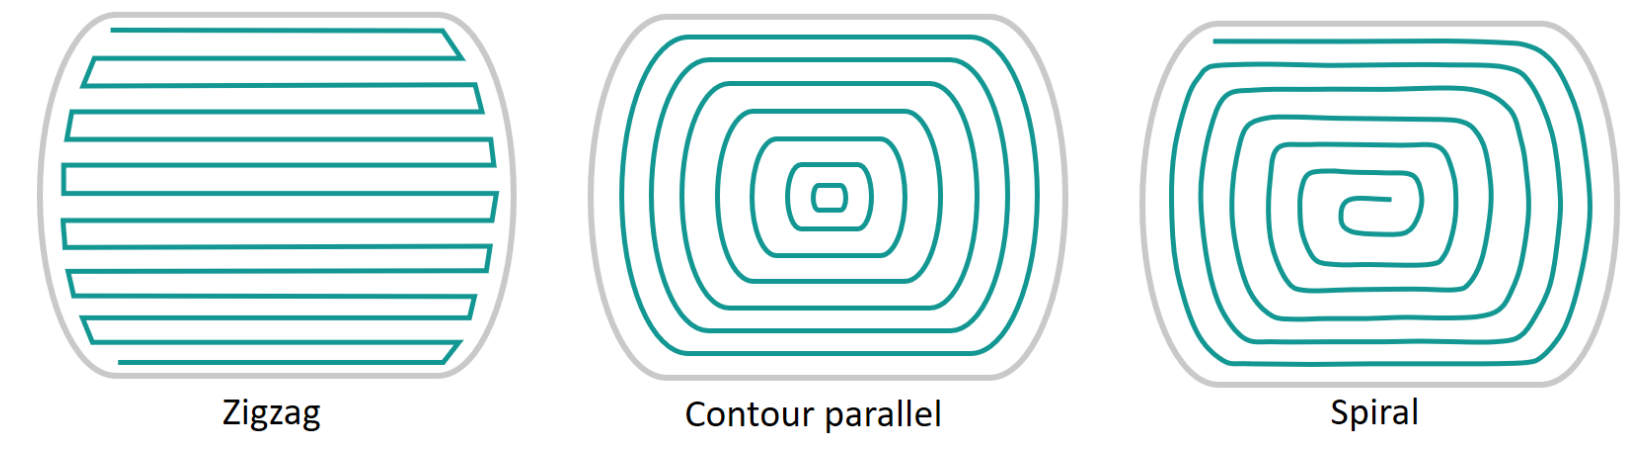
\includegraphics[scale=.35]{figures/path.png}}
	\caption{Three exemplary tool paths for iso-planar milling \cite{Zhao.2018}}
	\label{3path}
\end{figure}

\section{Optimization Algorithms}%

Optimization algorithms are computational methods used to find the best possible solution to a problem within a given set of constraints. These algorithms aim to minimize or maximize an objective function by iteratively adjusting the values of decision variables \cite{Sivanandam.2007b}. They are widely used in various fields, including engineering, operations research, finance, and machine learning, to optimize resource allocation, scheduling, parameter tuning, and other complex tasks. For the problem described in \ref{Problem Formulation} optimization algorithms can be used for determining optimal parameters for the redundant degrees of freedom while considering the defined objective, like reduction of direction changes or energy optimization. 


Optimization algorithms are computational techniques employed to identify the optimal solution or set of solutions for a given problem. There are several types of optimization algorithms, each exhibiting a unique methodology and characteristics.   Gradient-based optimization algorithms, like gradient descent, update the solution iteratively by following the direction of the steepest ascent or descent of the objective function \cite{Ruder.2017}. These algorithms are efficient for convex optimization problems where the objective function is smooth and has a unique global minimum or maximum.

Another type of optimization algorithm is the evolutionary algorithm, which is inspired by biological evolution. Evolutionary algorithms employ mutation, crossover, and selection to progressively shape a population of solutions over time. These techniques are especially applicable to resolving intricate optimization problems characterized by non-linear and non-convex objective functions. By reading a wider range of the search space, evolutionary algorithms can uncover tier-one solutions that draw near to the global optimum, although they may necessitate enhanced computational resources \cite{Back.1993}.

Particle swarm optimization (PSO) is a metaheuristic optimization algorithm based on the collective behavior of a particle swarm. In PSO, each particle represents a potential solution, and it moves through the search space to discover the optimal solution by exchanging information with nearby particles. This cooperative behavior enables the algorithm to efficiently converge to better solutions. PSO is especially beneficial for continuous optimization problems that have numerous local optima \cite{Back.1993}.

Genetic algorithms are evolutionary algorithms that use genetic operators, like crossover and mutation, to evolve solutions in a population. They can handle various types of optimization problems. Genetic algorithms are particularly effective for multi-objective optimization problems. They generate a set of solutions called the Pareto front, which represents the trade-off between conflicting objectives \cite{Lambora.2019,Katoch.2021}.

In recent years, there has been an increasing interest in metaheuristic optimization algorithms. Examples of such algorithms are ant colony optimization, differential evolution, and harmony search, which draw inspiration from natural phenomena or human behavior. These general-purpose algorithms can be applied to various optimization problems and provide efficient and flexible approaches to finding optimal solutions \cite{Yang.2011}.

Optimization algorithms prove to be formidable resources for uncovering optimal solutions to intricate issues. Be it via gradient-based means, evolutionary algorithms, metaheuristics, or other customized mechanisms. Optimization algorithms effectively fine-tune objectives, meet requirements, and refine decision-making processes across a broad spectrum of industries. The algorithm choice relies on the problem's characteristics, the available computational resources, and the desired balance between solution quality and computational efficiency.


\begin{comment}
\section{Machine Learning}%
\subsection{General Introduction to ML}
Machine Learning is a subfield of Artificial Intelligence (AI) that focuses on the development of algorithms and models that enable computers to learn from and make predictions or decisions based on data. It involves training a machine learning model using labeled or unlabeled data to recognize patterns, make predictions, or perform specific tasks without being explicitly programmed.

The core idea behind machine learning is to enable computers to learn and improve from experience. Instead of being explicitly programmed for every possible scenario, machine learning algorithms are designed to learn from examples and data, allowing them to make informed decisions or predictions.

There are several types of machine learning algorithms, including supervised learning, unsupervised learning, and reinforcement learning. In supervised learning, the algorithm is trained on labeled data, where the desired output is provided along with the input. The algorithm learns to map the input to the correct output by generalizing from the training data. Unsupervised learning, on the other hand, involves training the algorithm on unlabeled data, and it learns to find patterns or structures within the data without any specific target output. Reinforcement learning is a type of learning where an agent learns to make decisions in an environment by receiving feedback or rewards based on its actions.

Machine learning has numerous applications across various industries and domains. It is used in natural language processing, computer vision, recommendation systems, fraud detection, autonomous vehicles, healthcare, finance, and many other fields. Machine learning models can analyze large amounts of data, extract meaningful insights, and make predictions or decisions with high accuracy, leading to improved efficiency, personalized experiences, and enhanced decision-making.

In summary, machine learning is a field of AI that focuses on developing algorithms and models that enable computers to learn from data and make predictions or decisions. It involves training models using labeled or unlabeled data, allowing them to recognize patterns, generalize from examples, and perform tasks without explicit programming. Machine learning has a wide range of applications and is transforming industries by enabling automation, personalization, and intelligent decision-making.


\subsection{Key Areas Of ML}

Machine Learning (ML) encompasses various key areas that focus on different aspects of learning algorithms and their application. Here is a short summary of some key areas of ML:


Supervised Learning: In this area, ML algorithms learn from labeled training data to make predictions or classify new, unseen data. The algorithms are trained on input-output pairs, and their goal is to learn the underlying patterns or relationships in the data to generalize well on unseen examples.


Unsupervised Learning: Unsupervised learning deals with unlabeled data, where the ML algorithms aim to discover hidden patterns, structures, or relationships in the data. It can involve tasks such as clustering, dimensionality reduction, or anomaly detection.


Reinforcement Learning: This area focuses on training agents to make sequential decisions in an environment to maximize a reward signal. Reinforcement learning algorithms learn through trial and error, receiving feedback in the form of rewards or penalties based on their actions.


\subsection{ML for Optimization Problems}
Machine Learning (ML) has proven to be highly effective in solving optimization problems across various domains. Optimization problems involve finding the best solution from a set of possible solutions, often subject to certain constraints. ML techniques can be utilized to enhance the efficiency and accuracy of optimization algorithms, leading to improved outcomes.

One common approach is to use ML for parameter tuning in optimization algorithms. Many optimization algorithms require the selection of various parameters, such as learning rates, regularization factors, or population sizes. Traditionally, these parameters are manually chosen by experts through trial and error. ML techniques, such as grid search or Bayesian optimization, can automate the process of parameter tuning by searching through the parameter space and finding the best combination of parameters that optimize the objective function. This reduces the need for manual intervention and leads to better performance of the optimization algorithm.

Another way ML can be applied to optimization problems is through the use of surrogate models. Surrogate models are approximations of the objective function that are computationally cheaper to evaluate. ML algorithms, such as regression or Gaussian processes, can be used to build these surrogate models based on a small number of evaluations of the objective function. The surrogate models can then be used to guide the optimization algorithm, reducing the number of expensive evaluations of the objective function and speeding up the optimization process. This is particularly useful in scenarios where the objective function is time-consuming or expensive to evaluate, such as in engineering design or financial portfolio optimization.

ML can also be used to learn heuristics for solving optimization problems. Heuristics are problem-solving techniques or rules of thumb that are not guaranteed to find the optimal solution but often provide good approximate solutions. ML algorithms, such as genetic programming or reinforcement learning, can be employed to learn heuristics from data or experience. The ML model is trained on a set of problem instances and their corresponding solutions, and it learns to identify patterns or strategies that lead to good solutions. The learned heuristics can then be applied to new problem instances to find near-optimal solutions quickly.

Furthermore, ML can be used to solve combinatorial optimization problems. These problems involve finding the best arrangement or combination of elements from a finite set. ML algorithms, such as deep learning or graph neural networks, can be applied to learn the underlying structure or patterns in the problem domain. The ML model can then be used to guide the search for the optimal solution by predicting the quality or feasibility of different combinations of elements. This approach has been successfully applied to problems such as vehicle routing, resource allocation, or job scheduling, where finding the optimal solution is computationally challenging.

In conclusion, ML techniques offer powerful tools for solving optimization problems. By automating parameter tuning, building surrogate models, learning heuristics, or solving combinatorial optimization problems, ML can enhance the efficiency and accuracy of optimization algorithms. These advancements in ML for optimization problems have the potential to revolutionize industries such as logistics, manufacturing, finance, and many others by enabling faster, more accurate decision-making and resource allocation.
\end{comment}
\newpage
\section{Comparison of the State of the Art }%

In the following, a literature analysis is performed regarding the optimization of various process parameters. The focus lies on manufacturing systems with redundant degrees of freedom for tasks such as milling and WAAM. 
Table \ref{parameter} summarizes the analyzed parameters. 


\begin{table} [h!]
	\centering
	\begin{tabular}{|l|l|}
		\hline
		\hline
		Singularity avoidance \cite{Huo.2008} & Joint accelerations \cite{Gasparetto.2010}\\
		Joint jerks \cite{Gasparetto.2010} & Stiffness \cite{Cvitanic.2020} \\
		Energy use \cite{Paryanto.2015} & \\
		\hline
		\hline
		
	\end{tabular}
	
	
	\caption{Areas of influence of boundary conditions and process parameters}
	\label{parameter}
\end{table}

Additional parameters like transfer time, precision and maximum load capacity can also be analyzed but are omitted from the detailed analysis due to the limitation of scope \cite{Breaz.2017, Hirzinger.2005, Pham.2018}. Direction changes in the joint are briefly mentioned in \cite{Halbauer.2013} but not discussed in detail in any other publication.

\subsubsection{Singularity avoidance}
As mentioned in Chapter \ref{Problem Formulation}, Singularities occur when the robot manipulator loses control or achieves limited mobility due to certain configurations~\cite{Malyshev.2022}. This result in the loss of a DoF or make the system highly sensitive to small changes~\cite{Zhao.2021, Milenkovic.2021}.
Image \ref{wristsingular} shows how the 5th joint needs to rotate significantly when moving along a straight line in Cartesian space. 

\begin{figure}[H]
	\centerline{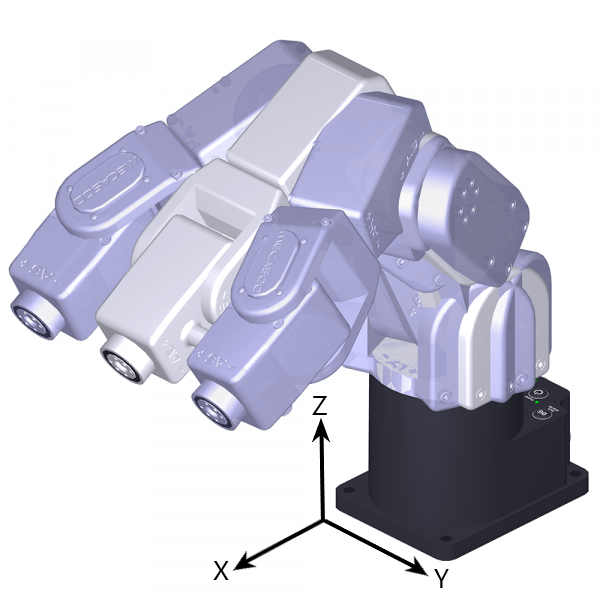
\includegraphics[scale=.25]{figures/wristsingular.png}}
	\caption{Passing trough a wrist singularity \cite{meca}}
	\label{wristsingular}
\end{figure}



Tasks that involve functional redundancy, as where the manipulator has more DoF than required for the task, the general projection method cannot be applied. Robotic industrial welding processes often have functional redundancy due to the presence of symmetry axes when using generic 6-DoF industrial robots. Different approaches have been proposed to solve functional redundancy, including adding a virtual joint to the manipulator or using the twist decomposition approach (TWA).

Most of the research is limited to the mathematical analysis of singularities and does not  consider the industrial implementation of the proposed algorithms in a industrial setting. The manipulability measure and maximization of Jacobian minors are commonly used methods to avoid singularities. Other methods such as condition number and singular value decomposition can also be used \cite{Stevenson.}. Another mathematical analysis performs a differentiation between non-recoverable singularities and reconfiguration by self motion into a nonsingular configuration is possible \cite{Bedrossian.2002}

Another approach proposes a kinetostatic performance index for evaluating the quality of robotic postures which includes singularity avoidance and joint limit consideration \cite{Huo.2008}. This method is also transferable to applications like milling. A parameter called "condition number" and "manipulability" is introduced which are used to calculate the "kinetostatic performance index". The presented method can increase the distance from singularities and lower the the maximum rotation velocity of the fourth joint. One disadvantage of the proposed method is the manual selection of a parameter. This parameter is responsible for avoiding the joint-limits and minimizing joint velocities. Manual fine-tuning of that parameter is required for optimal performance. 

Further approaches are introducing roll motion around the tool's symmetry axis to counter the loss of a degree of freedom at the singularity. Paths with varying tool roll or fixed roll angles can be chosen, with considerations for tool elevation changes and mechanical interference. Selecting paths with a fixed roll angle simplifies implementation for existing robot controllers \cite{Milenkovic.2021}.

\subsubsection{Optimization of Joint Accelerations and Jerk}

Jerk and accelerations control is critical because high values can wear out the robot structure and significantly stimulate its resonance frequencies. Vibrations caused by non-smooth trajectories can harm the robot's actuators and produce substantial deviations when completing tasks like trajectory tracking. Furthermore, low-jerk trajectories can be accomplished more quickly and precisely \cite{Gasparetto.2010}.
  
  
One recently published approach uses a adaptive greedy algorithm to generate the jerkoptimized trajectory with discrete time constraints. The proposed algorithm improves the trajectory in an iterative routine after obtaining an initial trajectory by a graph-search method \cite{Dai.2020}.
A further method  proposes a sequential quadratic programming method. The results show that optimal time-jerk trajectories which the traveling time constraints can be obtained \cite{Jiang.2017}. 
  
Another method is proposing a method of reconstructing the path by a sequence of via-points that define the positions and orientations of the robot's end-effector. Unlike most minimum-jerk trajectory planning techniques, this algorithm does not force an execution time beforehand and takes into account constraints such as upper bounds on velocity, acceleration, and jerk. The algorithm uses a hybrid objective function that balances execution time and smoothness of the trajectory. The output of the algorithm is a vector of time intervals between consecutive via-points that minimizes the objective function \cite{Gasparetto.2010}. 


\subsubsection{Optimization of Stiffens}

A recent publication is evaluating the stiffness of a robot using a newly defined performance index, which is maximized to optimize the robot's posture. The problem is solved using a discretization search algorithm, taking into account joint limits, singularity avoidance, and trajectory smoothness. 
Each joint of the robot is modeled as a linear torsion spring which are transferred into a stiffness matrix. This method is applied to a 6-DoF robot that is used for a milling operation. The goal of this 
method is to set the redundant angle  such that stiffness is maximized. Simulations and experiments on an industrial robot validate the performance index and optimization algorithm, demonstrating improved machining accuracy using this method \cite{Xiong.2019}.


Another approach is working with a dynamic model to reduce the regenerative chatter in a milling operation with a 6-DoF robot. By considering the frequency response function the limiting cutting depth can be determined. The cutting depth is a function of the redundant degree of freedom, which is the rotation around the axis of the spindle. A experimental analysis of o full-slut cut is performed. The results show that a significant reduction in chatter can be achieved by setting the redundant degree of freedom to the optimal value \cite{Wang.2022}.

A further publication performs a comparative study of robot pose optimization using static and dynamic stiffness models. The results suggest that static stiffness model can achieve close to optimal results for pose selection for tasks where the process forces do not approach the resonant frequencies of the robot. It is also discussed  that static and dynamic stiffness-based optimizations cannot reduce the deflections ot the cutting tool to a range smaller of the robot's repeatability \cite{Cvitanic.2020}.


\subsubsection{Optimization of Energy use}

It is shown that in a setting where a 6-DoF is used to perform a 5-doF task, energy savings up to 20.8\% can be expected. The proposed method is using the yaw angle as a optimization variable that can be set to a value in a certain range \cite{Boscariol.2020}. 

Another publication analyzes the general energy consumption of a industrial robot. The results show that cooling and the movement speed have the most significant impact on the energy consumption. The axis drives are responsible for 23\% of the energy consumption. Based on this result, it is shown that optimizing the robots movement in regards to optimal cycle time will significantly reduce its energy usage \cite{Uhlmann.2016}. 


\subsubsection{Summery}
Setting the appropriate process parameters directly impacts the performance and efficiency of a production system. By carefully fine-tuning parameters such as singularity avoidance, joint accelerations, and jerks, the system can operate smoothly, minimizing wear structure while achieving precise trajectory tracking. Moreover, optimizing energy usage through the adjustment of parameters related to movement speed not only contributes to environmental sustainability but also leads to economic benefits by reducing long-term operational costs. Additionally, the consideration of parameters like stiffness and joint limits ensures the safety of both the manufacturing system and its operators. The optimization of stiffness, for instance, enables the maximization of the system's performance and the attainment of improved machining accuracy. In conclusion, the careful selection and optimization of process parameters play a significant role in achieving optimal performance, efficiency, safety, and utilization of manufacturing systems, thereby contributing to overall operational success.